\section{Un modèle}
\label{sec:model}

Nous nous sommes ensuite intéressé à la location des renommages. Sont-ils plus proches des releases majeurs que des releases mineurs ? Nous nous sommes aussi demandé si Git détectais ces renommages au niveau des fichiers, et si celà pouvait être un indicateur pour tout les changements d'identités.\\
Nous avons donc décidés d'utiliser à partir de maintenant la detection de renommages de Git, afin de couvrir un grand nombre de commits dans plusieurs projets et plusieurs langages de programmation et donc nous fixer à un seul niveau de granularité, les fichiers.\\\\
Nous définissons maintenant le modèle \figref{model}, que les projets que nous allons analyser devrons respecter.\\\\
\begin{figure}[t]
  \centering
  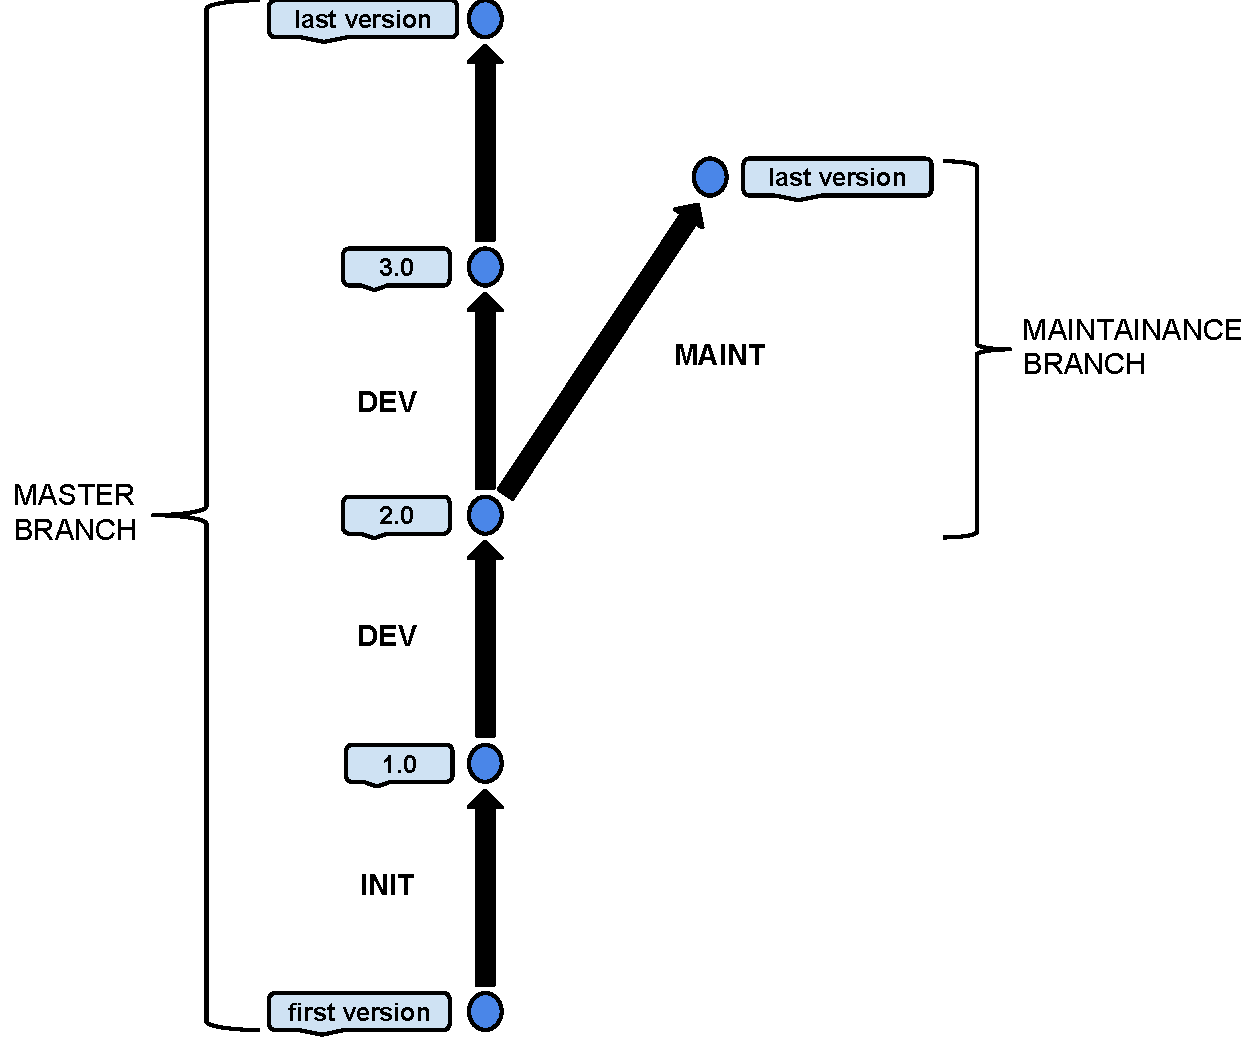
\includegraphics[scale=0.5]{data/figures/periods.pdf}
	\caption{Modèle d'architecture de dépot de code source}
	\label{fig:model}
\end{figure}
Ce modèle représente une architecture pour le dépot de code source dérivé de l'architecture Git Flow.\\
Les projets de développement logiciel suivent généralement des phases distinctes durant leur cycle de vie. Habituellement une période de développement commence avant qu'une première release soit accécible aux utilisateurs, puis cette release est maintenu pendant qu'une autre se prépare et ainsi de suite.\\   
Nous avons ainsi deux types de branches, les branches de maintenance et la branche master. Nous divisons les branches en périodes, c'est à dire en une séquence de commits, la branche master contient une période initial (init) entre la première version du logiciel (incluse) et la première release, puis des périodes de développement (dev) entre chaque releases. Chaque projet contient des releases majeurs, qui correspondes à des point clé du projet, des périodes susceptible de contenir beaucoup de changements, et des releases mineurs. On distingue les releases majeurs des mineurs par une augmentation significative du numéro de release. Par exemble $1.9-2.0$ pour Jquery, $3.7-4.0$ pour PHPUnit ou $0.13-1.0$ pour Rails. De l'autre côté les branches de maintenance sont divisés en périodes (maint) entre chaque releases.\\
 
